\section{Jagtudøvelse}

\begin{frame}
  \vspace{3em}
  \begin{center}
    {\LARGE \textbf{Bekendtgørelse af lov om jagt og vildtforvaltning}} \\
    \vspace{1em}
    LBK nr 639 af 26/05/2023, §§ 13-32
  \end{center}
\end{frame}

\begin{frame}{Jagtretten – grundregler (§13–§15)}
    \begin{itemize}
        \item \textbf{§13}: Ingen må jage uden jagtret – medmindre samtykke fra jagtberettiget
        \item \textbf{§14}: Jagtretten tilkommer ejendommens ejer
          \begin{itemize}
            \item På ferske vande (uden særlig ejendomsret): Ejerne af tilstødende ejendomme (nærmeste del)
            \item Gælder ikke hvis ældre rettigheder giver retten til andre
          \end{itemize}
        \item \textbf{§15}: Fast bopæl i DK → ret til ikke-erhvervsmæssig jagt på fiskeriterritoriet (fra højeste vandstandslinje)
          \begin{itemize}
            \item Gælder ikke hvis ældre ret til tilgrænsende landarealer
            \item Undtagelse: EU/EØS-borgere med tilknytning til DK
          \end{itemize}
    \end{itemize}
\end{frame}

\begin{frame}{Jagtretten – offentlig vej og tilegnelse (§16–§17)}
    \begin{itemize}
        \item \textbf{§16}: Forbud mod jagt på/fra offentlig vej eller sti
          \begin{itemize}
            \item Tilladt at tilegne sig beskudt vildt, der falder på vej/sti fra egen grund
          \end{itemize}
        \item \textbf{§17}: Beskudt vildt på egen grund → må ikke tilegnes hvis det falder på anden grund
          \begin{itemize}
            \item Underret snarest ejer/jagtberettiget
          \end{itemize}
    \end{itemize}
\end{frame}

\begin{frame}{Arealgrænser og minimumskrav (§18)}
    \begin{itemize}
        \item \textbf{§18}: Minimum 1 ha sammenhængende areal til jagt (vej/jernbane krydses OK)
          \begin{itemize}
            \item Fra 1 - 5 ha: Kun ejer + husstand (eller brugsret-indehaver + husstand)
            \item Aftale med tilgrænsende arealer → kan overstige grænser (naboaftale)
            \item Øer mindre end 1 ha: OK hvis jagt tilladt på omgivende fiskeriterritorium
            \item Fælleseje (flere end 4 ejere): Skriftlig aftale + 3/4 tilslutning
          \end{itemize}
    \end{itemize}
\end{frame}


\begin{frame}{Afstande, overdragelse og ældre rettigheder (§19–§21)}
    \begin{itemize}
        \item \textbf{§19}: Ingen skud inden for 50 m fra beboelsesbygninger (uden samtykke)
          \begin{itemize}
            \item På fiskeriterritoriet: 100 m fra sommerhusområde / 500 m fra byzone
          \end{itemize}
        \item \textbf{§20}: Jagtretten kan ikke afhændes særskilt/varigt fra ejendomsretten
          \begin{itemize}
            \item Overdragelse: Max 30 år ad gangen
            \item Ved brugsret-overdragelse: Jagtretten følger med (medmindre aftalt andet)
          \end{itemize}
        \item \textbf{§21}: Ældre rettigheder → ejer kan kræve afløsning (kapitaliseret jagtleje)
    \end{itemize}
\end{frame}



\begin{frame}{Jagtetik, sikkerhed og unge jægere (§22–§23)}
    \begin{itemize}
        \item \textbf{§22}: Ingen må jage på en måde, der
          \begin{itemize}
            \item udsætter vildtet for unødige lidelser
            \item skader personer, husdyr eller genstande eller udsætter personer for nærliggende fare
            \item medfører haglnedfald på anden persons bolig, have eller gårdsplads
          \end{itemize}
        \item \textbf{Stk. 2}: Personer under 18 år (med gyldigt jagttegn) må kun jage i følge med en person over 18 år (med gyldigt jagttegn)
        \item \textbf{§23}: Nedlæggelse/ombringelse af vildt må kun ske med skydevåben
          \begin{itemize}
            \item Rovfugle og ugler må ikke anvendes til jagt
            \item Jagt må ikke ske med levende lokkedyr
          \end{itemize}
    \end{itemize}
\end{frame}

\begin{frame}{Våbenkrav, hunde og jagt fra køretøj/fartøj (§24–§26)}
    \begin{itemize}
        \item \textbf{§24}: Ved jagt med glatløbet haglgevær på ikkeklovbærende vildt (på/fra landarealer, rør- og sivbevoksninger) skal egnet apporterende hund medbringes
        \item \textbf{§25}: Jagt må ikke finde sted fra motordrevet køretøj eller luftfartøj
        \item \textbf{§26}: Jagt fra motordrevet fartøj må ikke finde sted på søer og andre ferske vande
        \item \textbf{§23 stk. 4–6}: Ministeren fastsætter regler om
          \begin{itemize}
            \item tilladte våben/ammunition
            \item salg/medtagelse af visse ammunitionstyper
            \item brug af rovfugle, hjælpemidler, lokkemidler mv.
          \end{itemize}
    \end{itemize}
\end{frame}

\begin{frame}{Fodring, skjul, hegn og færdsel med våben (§28–§31)}
    \begin{itemize}
        \item \textbf{§28}: Udfodring af vildt med jagt for øje må ikke finde sted – vildt må ikke beskydes nær foderplads
          \begin{itemize}
            \item Ministeren kan fastsætte regler om fodring, foderpladser og placering
          \end{itemize}
        \item \textbf{§29}: Ministeren kan fastsætte regler om jagt fra platforme/kunstige skjul (inkl. forbud mod at medtage våben)
        \item \textbf{§30}: Hegn skal tillade ens passage af vildt fra begge sider (undtaget udsætningspladser, skovkulturer, veje/jernbaner)
        \item \textbf{§31}: Uvedkommende må ikke færdes med skydevåben/fangstredskaber på anden persons jagtgrund (undt. offentlige veje/stier)
          \begin{itemize}
            \item Gælder også i skove – kun på offentlige veje gennem skoven
            \item Naturbeskyttelseslovens adgangsregler giver ikke ret til at medbringe skydevåben/fangstredskaber
          \end{itemize}
    \end{itemize}
\end{frame}

\begin{frame}{Særlige jagtformer og anholdelsesbeføjelser (§27, §32)}
    \begin{itemize}
        \item \textbf{§27}: Ministeren kan fastsætte regler om jagtformer (herunder forbyde særlige former i bestemte områder)
        \item \textbf{§32}: Den jagtberettigede (eller dennes folk) må anholde enhver, der overtræder §13 (ulovlig jagt uden ret)
          \begin{itemize}
            \item Må føre den anholdte til politiet
            \item Samme beføjelse til arealet brugeren (selv uden jagtret) – skal underrette jagtberettiget
            \item Anholdte kan fratages skydevåben, redskaber og skudt/fanget vildt – afleveres straks til politiet (beslaglæggelse vurderes)
          \end{itemize}
    \end{itemize}
\end{frame}

\begin{frame}
  \vspace{3em}
  \begin{center}
    {\LARGE \textbf{Jagtudøvelse}
    }
    \\
    \vspace{1em}
    Bekendtgørelse om udsætning af vildt, jagtmåder og jagtredskaber
    \\
    \vspace{1em}
    BEK nr 1652 af 19/12/2017, Kapitel 2-5
  \end{center}
\end{frame}

\begin{frame}{Jagt i nærheden af indhegninger med hjorte (§4–§5)}
    \begin{itemize}
        \item \textbf{§4}: På ejendom med indhegnet hold af hjortedyr (jf. lov om hold af dyr)
          \begin{itemize}
            \item Vildtlevende individer af de opdrættede arter må \textbf{ikke} jages
            \item Gælder \textbf{i indhegningen} eller inden for \textbf{300 m} fra indhegningen
            \item Gælder også indhegninger, der er undtaget helt/delvist fra lov om hold af dyr (§19)
          \end{itemize}
        \item \textbf{§5}: På ejendom, hvor der \textbf{tidligere} har været holdt hjortedyr i indhegninger
          \begin{itemize}
            \item Hjortedyr må \textbf{ikke} jages \textbf{i indhegningen}
            \item Gælder hvis indhegningen (eller væsentlige dele) fortsat findes
          \end{itemize}
    \end{itemize}
\end{frame}



\begin{frame}{Jagt på fiskeriterritoriet – grundregler (§6)}
    \begin{itemize}
        \item \textbf{§6 stk. 1}: Den frie jagtret (jf. lovens §15) må kun udøves
          \begin{itemize}
            \item Fra flydende båd eller pram
            \item Fra areal, der grænser op til fiskeriterritoriet, hvor man har jagtret
          \end{itemize}
        \item \textbf{Stk. 2}: Færdsel med skydevåben under vadning på fiskeriterritoriet er \textbf{ikke tilladt}
        \item \textbf{Stk. 3} – Undtagelser (uanset stk. 1):
          \begin{itemize}
            \item Lovligt nedlagt vildt må indsamles ved vadning
            \item Rør- og sivbevoksninger må afdrives for vildt af den, der har jagtret på nærmeste tilgrænsende areal
          \end{itemize}
        \item \textbf{Stk. 4} – Vadning med skydevåben tilladt hvis:
          \begin{itemize}
            \item Skydevåbnet er \textbf{uladt}
            \item Vadning sker til/fra fartøj, ø eller holm med jagtret
            \item Ad korteste vej til sted, hvor våben lovligt kan medbringes (jf. §31)
          \end{itemize}
    \end{itemize}
\end{frame}

\begin{frame}{Fiskeriterritoriet}
    \begin{center}
        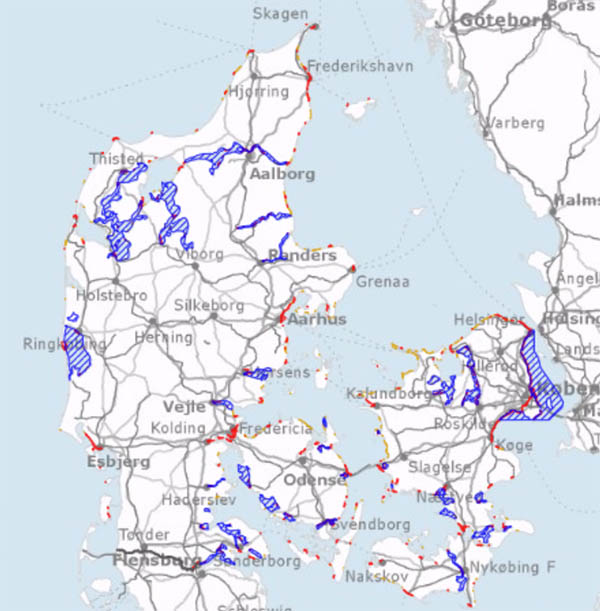
\includegraphics[width=0.45\textwidth]{Billeder/Andet/reservatkort.jpg}
        % Eller: [height=0.6\textheight] for højde-baseret skalering
    \end{center}
    
    % Her kan du tilføje tekst under billedet
    \vspace{1em}
    
\end{frame}

\begin{frame}{Jagt på fiskeriterritoriet – is og særlige begrænsninger (§7)}
    \begin{itemize}
        \item \textbf{§7 stk. 1}: På fiskeriterritoriet må der \textbf{ikke} drives jagt
          \begin{itemize}
            \item Fra is
            \item Inden for 100 m fra iskant
          \end{itemize}
        \item \textbf{Stk. 2}: Reglen i stk. 1 gælder \textbf{ikke} for jagt på \textbf{ræv}
    \end{itemize}
\end{frame}



\begin{frame}{Jagt fra båd – forbud og begrænsninger (§8)}
    \begin{itemize}
        \item \textbf{§8 stk. 1}: Der må \textbf{ikke} drives jagt fra motordrevet fartøj \textbf{i september måned}
        \item \textbf{Stk. 2}: Der må \textbf{ikke} drives jagt fra motordrevet fartøj
          \begin{itemize}
            \item på søer og andre ferske vande
            \item på de dele af fiskeriterritoriet, der er nævnt i \textbf{bilag 1} til bekendtgørelsen (vist på kortbilag)
          \end{itemize}
        \item \textbf{Stk. 3}: Der må \textbf{ikke} sejles med \textbf{ladt} skydevåben på tidspunkter/områder, hvor jagt ikke er tilladt
        \item \textbf{Stk. 4}: Miljøstyrelsen kan i særlige tilfælde dispensere fra stk. 2 (under iagttagelse af habitat- og fuglebeskyttelsesdirektivets artikel 16/9)
    \end{itemize}
\end{frame}

\begin{frame}{Jagt fra båd – hastighedsregler (§9)}
    \begin{itemize}
        \item \textbf{§9}: Til jagt må \textbf{ikke} benyttes motordrevet fartøj, der kan fremføres med mere end \textbf{18 km/t} (ca. 9,7 knob)
        \item Under selve jagtudøvelsen må fartøjet kun fremføres med højst \textbf{5 km/t} (ca. 2,7 knob)
        \item Husk kontekst:
          \begin{itemize}
            \item Generelt forbud mod jagt fra motordrevet fartøj på ferskvand (§26 i jagtloven)
            \item Begrænsede områder på fiskeriterritoriet (bilag 1-kort – ofte kystnære zoner, fjorde mv.)
            \item Ladt våben-forbud gælder uden for tilladte tidspunkter/områder
          \end{itemize}
    \end{itemize}
\end{frame}

\begin{frame}{Jagtmetoder – forbud på fiskeriterritoriet og ferske vande (§10)}
    \begin{itemize}
        \item \textbf{§10}: På fiskeriterritoriet og ferske vande må der \textbf{ikke} jages
          \begin{itemize}
            \item Kronvildt
            \item Dåvildt
            \item Sikavildt
            \item Råvildt
            \item Harer
            \item Mufloner
            \item Vildsvin
          \end{itemize}
        \item \textbf{Formål}: Beskytte store pattedyr og undgå ulovlig jagt i vandnære områder (supplerer generelle jagttider)
    \end{itemize}
\end{frame}

\begin{frame}{Forbudte hjælpemidler og jagtformer (§11–§12)}
    \begin{itemize}
        \item \textbf{§11}: Til jagt må \textbf{ikke} anvendes
          \begin{itemize}
            \item Mynder eller hunde af mynderacen
            \item Elektronisk udstyr til gengivelse af lyd (elektroniske lokkekald)
            \item Elektronisk udstyr til lokalisering af vildt (varmesøgende/termisk, lysforstærkende/natsigte)
            \item Kunstigt lys, spejle eller andre indretninger til belysning af målet
          \end{itemize}
        \item \textbf{§12}: På kronvildt er \textbf{tryk- og drivjagt} forbudt i perioderne
          \begin{itemize}
            \item 1. september – 15. oktober
            \item 1. februar – 29. februar
          \end{itemize}
        \item \textbf{Definition} (§12 stk. 2): Jagt hvor personer (med/uden hund) bevæger sig rundt og trykker/driver vildtet frem mod posterede skytter
    \end{itemize}
\end{frame}

\begin{frame}{Fodring af kronvildt (§13)}
    \begin{itemize}
        \item \textbf{§13 stk. 1}: Kronvildt må \textbf{ikke} fodres med valset korn eller kraftfoder
        \item \textbf{Stk. 2}: Øvrig fodring af kronvildt skal ske i mindst \textbf{130 m} afstand fra
          \begin{itemize}
            \item Platforme og skydestiger (jf. §1 stk. 2)
            \item Anden ejendom
          \end{itemize}
        \item \textbf{Stk. 3} – Undtagelse: Fodring nærmere end 130 m fra anden ejendom tilladt på ejendomme, hvor ejeren \textbf{ikke} har overdraget jagtretten på kronvildt til andre
        \item Husk: Generelt forbud mod udfodring med jagt for øje (§28 i bekendtgørelsen)
    \end{itemize}
\end{frame}